% Checked with Grammarly - 22/03/2021

\chapter{Design Overview}

This chapter describes a high-level design overview of the VisiBot Processing System and Interactive Web Application, highlighting the various design patterns, principles, and methods applied. 

\section{The VisiBot Processing System}

\subsection{Honeypot Integration}

The VisiBoT Processing System employs a wide network of honeypots, strategically distributed across a diverse set of network providers located in North America, South America, Asia, Europe, and Australia. The honeypot servers have been configured to emulate that of commonly targeted IoT devices, to maximise incoming botnet scanning activity and intrusion attempts. Once a honeypot detects an intrusion attempt, the corresponding packet information is sent to a central processing server for analysis and storage. Once received, the central honeypot processing server analyses and classifies packets based on characteristics observed across various Common Vulnerability Exploits (CVE). By analysing the payload string, post data, and TCP sequences of incoming packets, the honeypot service can infer which CVEs are being exploited by matching string patterns. Once processed, the captured honeypot packets are made accessible through a REST API (Application Protocol Interface) accessible by the VisiBot Processing System.

\subsection{Broker-based Packet Analysis}

The packets collected from the external honeypot service are processed and analysed in parallel, enabling real-time and efficient malware extraction and traffic classification. Real-time analysis is achieved through the adoption of the Message Broker architectural design pattern. Also known as Integration Broker, a Message Broker is "a third-party intermediary that facilitates interactions between applications" \citep{IBDefinition}, through the communication and transformation of messages between various independent programs by interacting with message broker through an API. A broker-based analysis system allows for the execution of time-consuming tasks to be distributed across multiple worker processes. As workers are completely separate from the main application and interact with a broker through an API, they can be reliably scaled and distributed across multiple systems. Clients, such as the VisiBot Processing System's main process, can connect to a broker and add, remove, or prioritise tasks. Connected workers actively consume and perform tasks from a central priority queue. 

Once a packet is received, the main VisiBot process creates a new packet analysis task, passing the task name and packet contents to the message broker to be later processed by a worker. The first stage of analysis involves malware payload URL extraction from the payload and post\_data contents of the packet. The URLs used in remote code execution requests or downloading and infecting devices can be extracted using a combination of Regular Expression and sub-string extraction techniques. If no strings match common URL regex patterns, such as \texttt{https?:}, then the attacker may be obfuscating URLs through command-line tool argument sub-strings. This prevents the automatic scraping of malware URL and requires URLs to be rebuilt from parsed argument strings. Through parsing the arguments of command-line tools commonly used for downloading binaries, such as \texttt{wget, curl} and \texttt{tftp}, the processing system can extract important sub-strings. Such strings include arguments such as IP addresses, domains, paths, and ports, which are used to reconstruct a full URL.

After all potential malware URLs are extracted, the worker will perform packet classification using the URL extraction process's information. Assuming a URL's corresponding IP address matches that of the packet's source IP address, the entity caught within the honeypot is deemed a malicious, self-propagating bot that self-hosts malware and actively performs port scanning and attacks on vulnerable devices. If the URL's IP address does not match the source IP of the packet, the processing system infers that the source packet IP corresponds to a Report Server. Unlike malicious bots, report servers separate entities used to infect vulnerable devices reported by infected bots. The IP corresponding to the extracted URL is therefore classified as a Payload server used by the Report Server to download and execute malware from within infiltrated devices. If no URLs are extracted, the packet's TCP sequence and target port are checked for port-scanning characteristics. As the Mirai botnet includes a TCP sequence within port-scanning requests, this sequence is used to infer if the packet resembles that of Mirai-like scanning activity. The request's targeted port is also used to infer if the packet matches that of generic botnet port-scanning activity, such as the sniffing of open telnet ports 23 and 2323. If any scanning activity is identified, the packet's source IP is classified as a "Bot", a benign botnet entity. Otherwise, the packet is deemed insignificant and is discarded. Following this, the worker will begin to collect information for all classified IP addresses, including the geographic location, WHOIS lookup information, proxy/tor/VPN detection, etc... The relationships between IP addresses are also recorded. For example, the interaction between a Report server and Payload server is stored as a directional graph where each IP address is represented as a node.

The worker's final stage of the analysis task is to request a malware analysis task of the extracted URL(s) by sending an API request to a remotely hosted malware sandbox service. Pending malware analysis tasks are logged in a database, allowing the system to manage and process incoming malware analysis reports from the external sandbox. Once the analysis is complete, the VisiBot Processing System will receive a malware analysis report through a Web API and process it accordingly. An overview of the interaction between the VisiBot Processing System and sandboxing service is depicted below:

\begin{figure}[!htb]
    \centering
    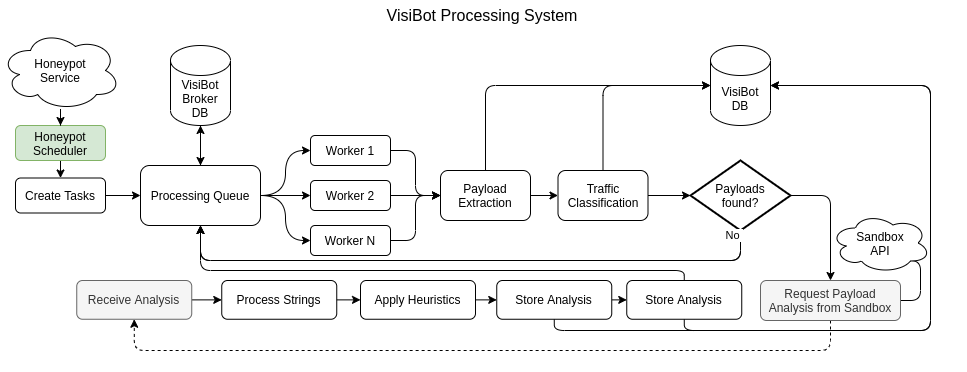
\includegraphics[width=0.8\linewidth]{flowcharts/high_level_processing_overview.png}
    \caption{High-level flow-diagram of the core VisiBot Processing System.}
    \label{fig:high_level_proc_overview} 
\end{figure}

\subsection{Scalable Sandboxing Service}

Like that of the VisiBot Processing System, the sandbox analysis system employed by VisiBot also utilises the Message Broker architectural design pattern. The VisiBot Processing System's tasks are performed by several scalable and distributable workers, allowing for real-time malware analysis. Hosted on a separate server from VisiBot, all malware samples are stored within a secure block-storage partition separate from the rest of the system. Upon receiving an analysis request from an external source, such as VisiBot, the sandboxing system will attempt to download and analyse a binary from the URL given in the request. If downloaded successfully, the main process will move the binary to a secure block-storage partition with limited file-system permissions, completely separate from the main system, and an analysis task will be added to the sandbox broker queue.

When a worker consumes an analysis task, a three-stage analysis process is performed on the binary. The first stage involves static analysis, in which information such as the target CPU architecture, endianess, and source-code strings of the binary is extracted. Following this, the binary is copied to a virtual machine instance running an embedded Linux operating system. The image used by the Virtual Machine (VM) is selected based on the detected CPU architecture of the binary. Several CPU architectures are supported, including MIPS, ARM, i386, aarch64, and x86/64, all of which are common to targeted IoT devices. Once a new Virtual Machine instance is created, the malware binary is executed and monitored for 30 seconds, after which the virtual machine is reset. During the monitoring procedure, dynamic and network analysis are performed, logging all incoming and outgoing network traffic, processes opened files, and system calls generated by the malware sample. This information is used to generate and send a report to the VisiBot Processing System following task completion. The report includes various relevant static, dynamic, and network information, including port usage statistics, DNS queries, HTTP requests, and hard-coded binary strings. Additionally, the sandbox also generates log and pcap files which can be used for further analysis. 

\begin{figure}[!htb]
    \centering
    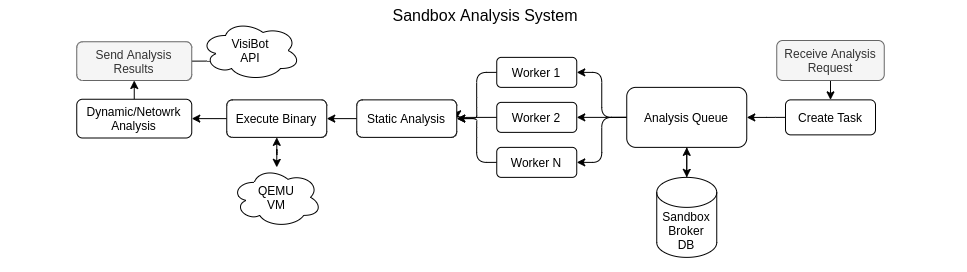
\includegraphics[width=0.8\linewidth]{flowcharts/high_level_sandbox_overview.png}
    \caption{High-level flow-diagram of malware sandbox analysis system.}
    \label{fig:high_level_sandbox} 
\end{figure}

\subsection{Heuristic Analysis}

Once VisiBot receives a malware analysis report from the sandboxing service, heuristic analysis is performed on the sample report to identify candidate Command \& Control servers and Peer-to-Peer botnet activity. The first heuristic is concerned with identifying Peer-to-Peer botnet activity through analysis of DNS queries performed during network analysis. All logged DNS queries are matched against a list of domain names corresponding to Peer-to-Peer Distributed Hash Table services, including commonly used public services offered by bittorrent.com, transmissionbt.com, and utorrent.com. Modern P2P Botnets, such as Mozi, connect to public DHT services to mask peer-to-peer botnet interactions amongst legitimate peers. Thus, the identification of such public DHT DNS names is ideal for inferring the presence of peer-to-peer botnet traffic. 

The second heuristic considers all transactional interactions with public IP addresses as potential C2/P2P activity. A transaction occurs when bytes are both sent to and received from an endpoint. Such data transactions are significant when identifying botnet traffic, as devices infected with botnet malware often attempt to perform handshakes and download updates/binaries from Command \& Control servers, Payload servers, or peer-to-peer botnet nodes.

The third heuristic combines entities of static and dynamic analysis. If any hard-coded IP addresses extracted during static analysis are later connected to during network analysis, the IP address is associated with a C2 server. Lastly, the fourth heuristic uses external IP blacklist services to infer that any IP address endpoints logged during network analysis previously blacklisted for Command \& Control activity are deemed malicious and are considered potential C2 servers. Once candidate C2 servers and P2P Nodes have been identified, the meta-data for each IP address is stored similarly to that of the first-stage classification process, storing geographical information, ASN records, etc. However, as the above heuristics are limited to the detection of \textit{candidate} botnet servers, all endpoints must be further validated through proper handshake confirmation procedures. This process is yet to be implemented within the VisiBot Processing System. However, the system can be easily extended to do so. The modularity of the system, provided by broker-based task processing, ensures that additional analysis stages can be added to the VisiBot Processing System with ease. For a full high-level overview of the VisiBot Processing System, including remote sandbox integration, see Appendix \ref{appendix_a0}.


\section{Interactive Web Application}

To allow for real-time visualisation of the botnets detected by the VisiBot Processing System, an interactive web-based application is used to display the geographic coordinates of all botnet entities identified within the last 24 hours of monitoring. Using the geographic coordinates collected during IP address meta-data collection, botnet entities are pinned onto a world-map, using a specific colour to represent different entities, such as Bots, Report servers, C2 servers, and P2P nodes. A variety of information is sourced directly from the VisiBot database and can be viewed through a front-end web interface that communicates with a back-end web server:

\begin{figure}[!htb]
    \centering
    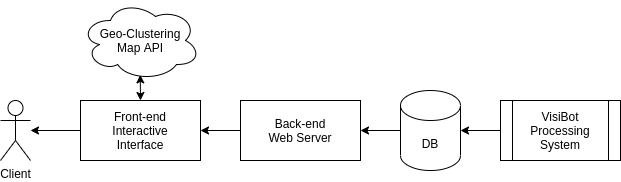
\includegraphics[width=0.6\linewidth]{flowcharts/design_overview_webapp.png}
    \caption{High-level overview of the VisiBot Web Interface.}
    \label{fig:webapp_design_overview} 
\end{figure}

Due to the amount of graphics being re-rendered whenever the map is updated, plotting thousands of geographic coordinates on a single world-map can result in high resource usage. A greedy geographic clustering algorithm is used to cluster coordinates into groups based on the geographic distance between points, mitigating visualisation performance issues:

\begin{lstlisting}[caption={Pseudocode for Greedy clustering algorithm based on an example by \citet{MarkerClustering}}]
foreach marker:
    if any cluster within cluster_distance of marker
        join(marker, cluster)
    else if any unclustered marker within cluster_distance of marker          create_cluster(marker, unclustered_marker)
\end{lstlisting}

Once clustered, the marker clusters are drawn in the map in-place of individual markers. When selected, the map will zoom in and un-cluster markers outside of the specified clustering distance. When a marker is selected, the visitor can view details about the entity and visualise its relationships with other entities recorded by VisiBot.



